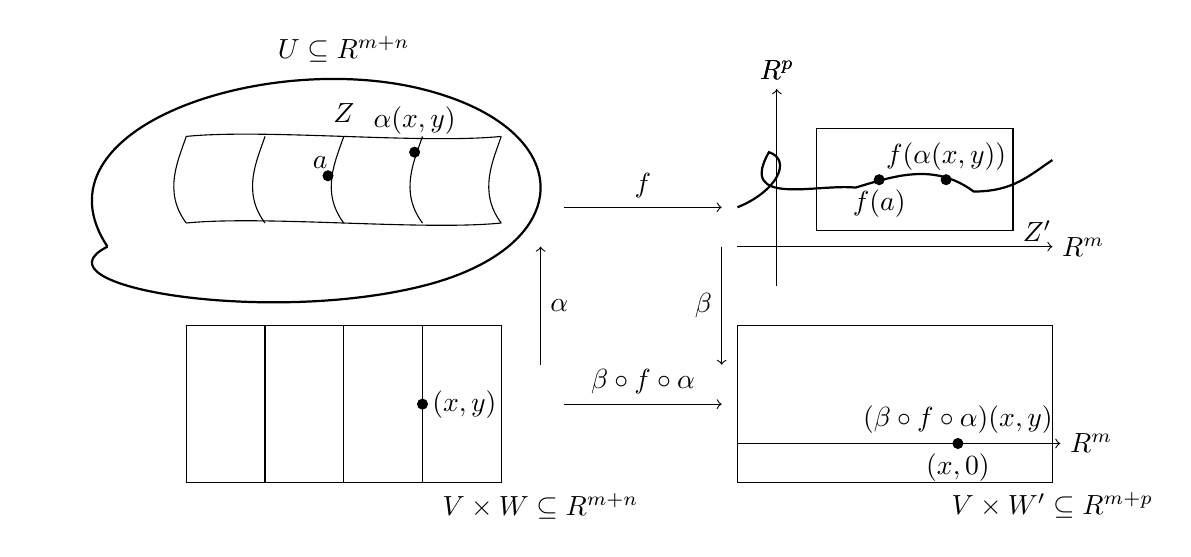
\begin{tikzpicture}[scale=1]

% ======================
% REGIÓN SUPERIOR (U)
% ======================

% Contorno tipo "orgánico"
\draw[thick] (-7,1.5) .. controls (-8,3) and (-5,4) .. (-3,3.5)
             .. controls (-1,3) and (-1,1.5) .. (-3,1)
             .. controls (-5,0.5) and (-8,1) .. (-7,1.5);

\node at (-4,4) {$U\subseteq \mathbb{R}^{m+n}$};
\node at (-4,3.2) {$Z$};

% "Fibras" (curvas horizontales suaves)
\foreach \y in {1.8,2.9} {
    \draw (-6,\y)
    .. controls (-5,{\y+0.1}) and (-3,{\y-0.1}) ..
    (-2,\y);
}

% Líneas verticales (estructura tipo producto)
\draw (-5,1.8)
.. controls (-5.3,2.2) and (-5.1,2.6) ..
(-5,2.9);

\draw (-4,1.8)
.. controls (-4.3,2.2) and (-4.1,2.6) ..
(-4,2.9);

\draw (-3,1.8)
.. controls (-3.3,2.2) and (-3.1,2.6) ..
(-3,2.9);

\draw (-6,1.8)
.. controls (-6.3,2.2) and (-6.1,2.6) ..
(-6,2.9);

\draw (-2,1.8)
.. controls (-2.3,2.2) and (-2.1,2.6) ..
(-2,2.9);


% Punto alphaxy
\fill (-3.1,2.7) circle (2pt);
  \node[above] at (-3.1,2.8) {$\alpha(x,y)$};

% Punto a
\fill (-4.2,2.4) circle (2pt);
\node[above] at (-4.3,2.37) {$a$};

% ======================
% REGIÓN INFERIOR (V x W)
% ======================

\draw (-6,-1.5) rectangle (-2,0.5);
\node at (-1.5,-1.8) {$V\times W\subseteq \mathbb{R}^{m+n}$};
% Grid
\foreach \x in {-6,-5,-4,-3,-2} {
    \draw (\x,-1.5) -- (\x,0.5);
}


% Punto (x,y)
\fill (-3,-0.5) circle (2pt);
  \node[right] at (-3,-0.5) {$(x,y)$};

% Flecha h
\draw[->] (-1.5,0) -- (-1.5,1.5);
\node[right] at (-1.5,0.75) {$\alpha$};


% ======================
% LADO DERECHO (R^n)
% ======================

\draw[->] (1.5,1) -- (1.5,3.5);
\node[above] at (1.5,3.5) {$\mathbb{R}^p$};

\draw[->] (1,1.5) -- (5,1.5);
\node[right] at (5,1.5) {$\mathbb{R}^m$};

\fill (2.8,2.35) circle (2pt);
\node[below] at (2.8,2.35) {$f(a)$};

\fill (3.65,2.35) circle (2pt);
\node[above] at (3.65,2.35) {$f(\alpha(x,y))$};

% Rectángulo (W)
\draw (2,1.7) rectangle (4.5,3);
\node[right] at (4.5,1.7) {$Z^{\prime}$};
  
% Curva dentro
\draw[thick] 
  (1,2) 
  .. controls (1.5,2.2) and (1.7,2.6) .. (1.4,2.7)
  .. controls (1,2) and (2,2.3) .. (2.5,2.25)
  .. controls (3,2.4) and (3.5,2.57) .. (4,2.2)
  .. controls (4.5,2.2) and (4.7,2.4) .. (5,2.6);
 
% Flecha f diagonal
\draw[->] (-1.2,2) -- (0.8,2);
\node[above] at (-0.2,2) {$f$};

% Flecha horizontal
\draw[->] (-1.2,-0.5) -- (0.8,-0.5);
\node[above] at (-0.2,-0.5) {$\beta\circ f\circ \alpha$};

% Flecha beta
\draw[->] (0.8,1.5) -- (0.8,0);
\node[left] at (0.8,0.75) {$\beta$};

% Rectangulo final

\draw (1,-1.5) rectangle (5,0.5);
\node[below] at (5,-1.5) {$V\times W^{\prime}\subseteq \mathbb{R}^{m+p}$};

\draw (1.5,1) -- (1.5,3.5);
\node[above] at (1.5,3.5) {$\mathbb{R}^p$};

\draw[->] (1,-1) -- (5.1,-1);
\node[right] at (5.1,-1) {$\mathbb{R}^m$};

\fill (3.8,-1) circle (2pt);
\node[below] at (3.8,-1) {$(x,0)$};
\node[above] at (3.8,-1) {$(\beta\circ f\circ \alpha)(x,y)$};

\end{tikzpicture}
